\problemname{Candy Necklace}
Alice wants to share a candy necklace with Bob.
The necklace consists of white and blue candies.
To be fair, Alice wants to split the necklace into two
parts with an equal number of candies in each.
However, Alice likes the blue candies much more than the white ones,
and therefore wants to get as many blue candies in her half as possible.

What is the largest number of blue candies Alice can get in her part,
if she cuts the necklace optimally?

\section*{Input}
The input consists of one line with a string describing the necklace.
The string consists only of the letters \texttt{B} and \texttt{V},
and has an even total number of letters.

\section*{Output}
Print a line with an integer: the maximum number of blue candies Alice
can get in her part of the necklace.

\section*{Scoring}
Your solution will be tested on a set of test groups.
To earn points for a group, you must pass all test cases in that group.

\noindent
\begin{tabular}{| l | l | p{12cm} |}
  \hline
  \textbf{Group} & \textbf{Points} & \textbf{Constraints} \\ \hline
  $1$   & $20$       & The necklace looks like in figure \ref{fig:group-1}. \\ \hline
  $2$   & $40$       & The necklace consists of at most $1\,000$ candies. \\ \hline
  $3$   & $40$       & The necklace consists of at most $10^6$ candies. \\ \hline
\end{tabular}


\begin{figure}[h]
	\centering
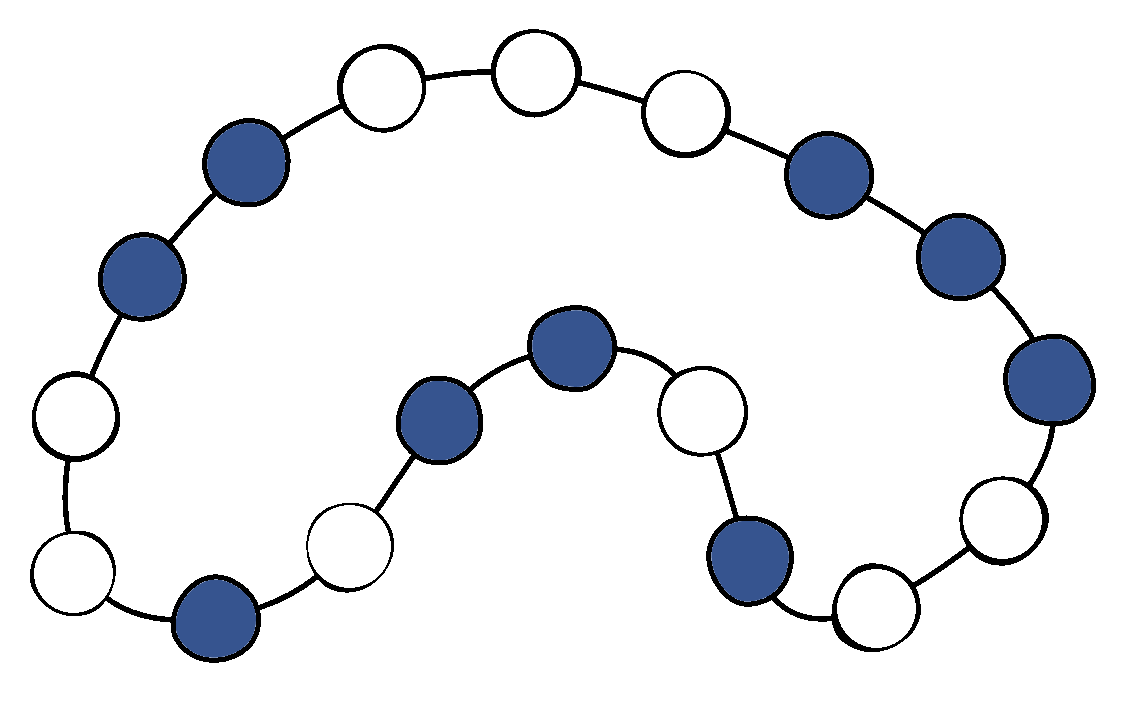
\includegraphics[width=0.5\textwidth]{group1}
\caption{The necklace in the first test group}
\label{fig:group-1}
\end{figure}


\section*{Explanation of Sample 1}
\texttt{BBVVBVVVBB} has length 10 so Alice must split the necklace into two parts with $5$ candies in each.
The possible parts she can get are \texttt{BBVVB}, \texttt{BVVBV}, \texttt{VVBVV}, \texttt{VBVVV},
\texttt{BVVVB}, \texttt{VVVBB}, \texttt{VVBBB}, \texttt{VBBBB}, \texttt{BBBBV}, \texttt{BBBVV}.
She gets the most blue candies by choosing \texttt{VBBBB} or \texttt{BBBBV} which have $4$ blue candies.



\begin{figure}[h]
	\centering
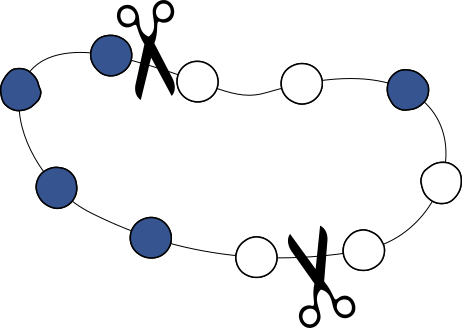
\includegraphics[width=0.5\textwidth]{sample1}
\caption{One of two optimal ways to cut in sample 1}
\end{figure}
